%+++++++++++++++++++++++++++++++++++++++++++++++++++++++++++++++
% SUMMARY    : Vectors, Matricies, Distance and Norms 
%            : University of Southern Maine 
%            : @james.quinlan
%            : Sarah Lawrence  - Lecture 3
%+++++++++++++++++++++++++++++++++++++++++++++++++++++++++++++++
\section*{Objectives}
\begin{itemize}
  \item Dimensionality - Code Examples
  \item Distance Explination
  \item Introduction to K-NN
  \end{itemize}

\rule[0.0051in]{\textwidth}{0.00025in}
% ----------------------------------------------------------------

\section{Review}
\[
\vec{x} \in {\mathbb{R}}^p
\]
Break down: 
\begin{itemize}
    \item $\vec{x}$ represents a vector. 
    \item $\in$ represents an element belonging to a particular set. 
    \item $\mathbb{R}$ represents all real numbers. 
    \item $p$ represents the dimension of the vector space. 
    \item \textbf{Meaning}: $\vec{x}$ is a vector with all elements being real numbers in $p$-dimensional space. 
    \item \textbf{Terminology}: $p$ can have other names such as Feature Space, and Factors.
\end{itemize}

Example: Column vector:
$\vec{x} = \begin{bmatrix}
x_1 \\
x_2 \\
\vdots \\
x_p
\end{bmatrix}$ \\

\[
    d(x,y)
\]
\textbf{Distance metric}: Measures the distance (dissimilarity) between two points x and y. 

\[
    d(x,y) = ||x-y||
\]
\textbf{Euclidean distance}: This is a specific type of distance metric. The straight line distance between two points in an Euclidean space. 

\[
    p>>1
\]
\textbf{Meaning}: This is $p$ much greater than one. If this happens then vector x has a high number of dimensions. \\
\textbf{Problem}: High dimensionality is called the ``Curse of Dimensionality". \\\\

\section{Lecture}
\subsection{Dimensionality}

Two dimensional vector space:


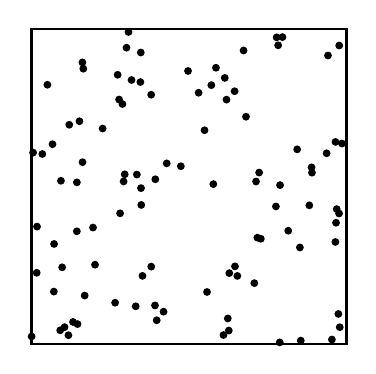
\begin{tikzpicture}
  % Draw the box
  \draw[thick] (0,0) rectangle (4,4); 

  % Generate random dots inside the box
  \foreach \i in {1,...,100} {
    \node[circle, fill=black, inner sep=1pt] at ({4*rnd}, {4*rnd}) {};
  }
  
\end{tikzpicture}


\textbf{Curse of Dimensionality}: When working in high-dimensional spaces it causes challenges. Such challenges include data sparsity and overfitting in machine learning. \\

Example:  High dimensionality (p value) in a two dimensional space.\\

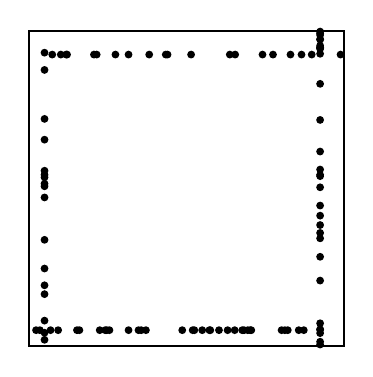
\begin{tikzpicture}
  % Draw the 4x4 box
  \draw[thick] (0,0) rectangle (4,4); 

  % Generate random dots near all four edges
  \foreach \i in {1,...,100} {
    \pgfmathsetmacro{\edgeSelector}{int(rnd*4)} 
    \pgfmathsetmacro{\pos}{rnd*4} 

    \ifnum \edgeSelector=0
      \node[circle, fill=black, inner sep=1pt] at (\pos, 0.2) {}; % Bottom edge
    \else
      \ifnum \edgeSelector=1
        \node[circle, fill=black, inner sep=1pt] at (\pos, 3.7) {}; % Top edge
      \else
        \ifnum \edgeSelector=2
          \node[circle, fill=black, inner sep=1pt] at (0.2, \pos) {}; % Left edge
        \else
          \node[circle, fill=black, inner sep=1pt] at (3.7, \pos) {}; % Right edge
        \fi
      \fi
    \fi
  }
\end{tikzpicture}\\\\
\textbf{Dimensionality Reduction}: reduce the number of dimensions in a dataset while retaining as much of the relevant information as possible. \\

Example: From three dimensions to two dimensions.

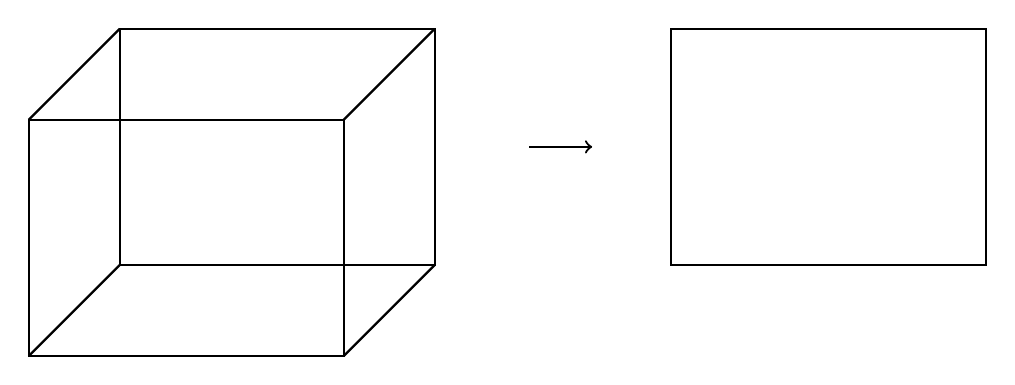
\begin{tikzpicture}

% Coordinates
\coordinate (A) at (0,0,0);
\coordinate (B) at (4,0,0);
\coordinate (C) at (4,3,0);
\coordinate (D) at (0,3,0);
\coordinate (E) at (0,0,3);
\coordinate (F) at (4,0,3);
\coordinate (G) at (4,3,3);
\coordinate (H) at (0,3,3);

% Box lines
\draw[thick] (A) -- (B) -- (C) -- (D) -- cycle; % Bottom
\draw[thick] (E) -- (F) -- (G) -- (H) -- cycle; % Top
\draw[thick] (A) -- (E);
\draw[thick] (B) -- (F);
\draw[thick] (C) -- (G);
\draw[thick] (D) -- (H);

\begin{scope}[shift={(7,0)}]
    % 2D box 
    \draw[thick] (0,0) rectangle (4,3); 
    \node at (2,1.5) {};
\end{scope}

\draw[->, thick] (5.2, 1.5) -- (6, 1.5);

\end{tikzpicture} 

What is the size of the box $\ell$ that always has $k$ number of dots in it? \\
Breakdown: 
\begin{itemize}
    \item $k$ = fixed number $<$ $n$ (red dots)
    \item $n$ = number of samples (pink dots)
    \item $p$ = dimensions
    \item Terminology: If $p$ is $\geq 4$ it's a \textbf{hyper-cube}
\end{itemize}

Example: $k = 1$, $p = 1$, $n = 3$ 
\begin{center}
    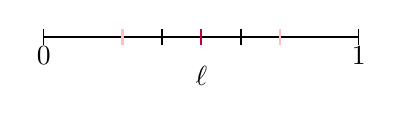
\begin{tikzpicture}
        % Draw the line segment
        \draw[thick] (0,0) -- (4,0);
    
        % Add labels at 0 and 1
        \node[below] at (0,0) {0};
        \node[below] at (4,0) {1};
    
        % Draw small ticks at 0 and 1
        \draw (0,0.1) -- (0,-0.1);
        \draw[thick, pink] (1,0.1) -- (1,-0.1);
        \draw[thick] (1.5,0.1) -- (1.5,-0.1);
        \draw[thick, purple] (2,0.1) -- (2,-0.1);
        \draw[thick] (2.5,0.1) -- (2.5,-0.1);
        \draw[thick, pink] (3,0.1) -- (3,-0.1);
        \draw (4,0.1) -- (4,-0.1);
    
        \node at (2, -0.5) {$\ell$}; % Bottom label
    \end{tikzpicture}
\end{center}

Example: $k = 3$, $p = 2$, $n = 100$ 
\begin{center}
    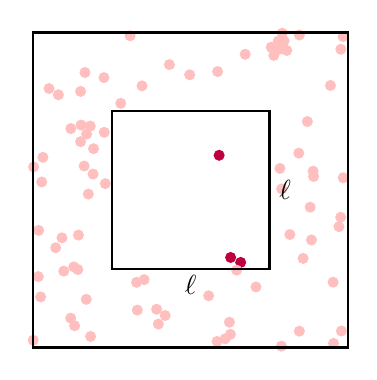
\begin{tikzpicture}
    
      % Generate 3 fixed dots inside the inner square
    \foreach \i in {1,2,3} {
        \pgfmathsetmacro{\x}{1 + rnd*2} % Random x between 1 and 3
        \pgfmathsetmacro{\y}{1 + rnd*2} % Random y between 1 and 3
        \fill[purple] (\x,\y) circle (2pt);
    }
    
    % Generate 50 random dots outside the inner square but within the big box
    \foreach \i in {1,...,100} {
        \pgfmathsetmacro{\x}{rnd*4} % Random x within the outer box
        \pgfmathsetmacro{\y}{rnd*4} % Random y within the outer box
        % Ensure points are outside the inner box
        \ifdim \x pt < 1 pt \fill[pink] (\x,\y) circle (2pt);
        \else \ifdim \x pt > 3 pt \fill[pink] (\x,\y) circle (2pt);
        \else \ifdim \y pt < 1 pt \fill[pink] (\x,\y) circle (2pt);
        \else \ifdim \y pt > 3 pt \fill[pink] (\x,\y) circle (2pt);
        \fi\fi\fi\fi
    }
    
      \node at (2, 0.8) {$\ell$}; % Bottom label
      \node at (3.2, 2) {$\ell$};  % Right label
      
      % Draw the box
      \draw[thick] (0,0) rectangle (4,4); 
    
      \draw[thick] (1,1) rectangle (3,3);
      
    \end{tikzpicture} 
\end{center}

\pagebreak % to align description with the tikz image

Example: $k = 3$, $p = 3$, $n = 100$
\begin{center}
    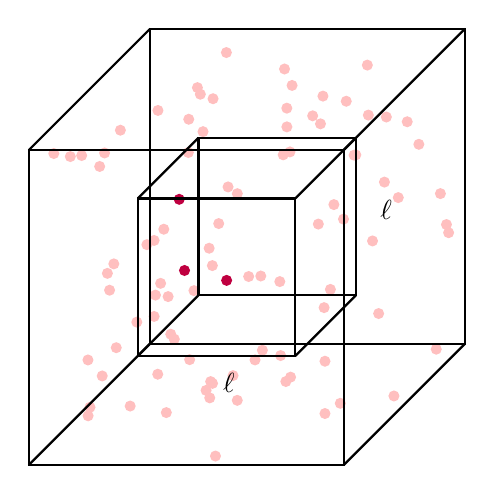
\begin{tikzpicture}
    
    % Generate random dots inside the outer box
    \foreach \i in {1,...,100} {
        \pgfmathsetmacro{\x}{rnd*4} % Random x between 0 and 4
        \pgfmathsetmacro{\y}{rnd*4} % Random y between 0 and 4
        \pgfmathsetmacro{\z}{rnd*4} % Random z between 0 and 4
    
        % Ensure the dot is strictly outside the inner cube
        \ifdim \x pt < 1 pt \fill[pink] (\x,\y,\z) circle (2pt);
        \else \ifdim \x pt > 3 pt \fill[pink] (\x,\y,\z) circle (2pt);
        \else \ifdim \y pt < 1 pt \fill[pink] (\x,\y,\z) circle (2pt);
        \else \ifdim \y pt > 3 pt \fill[pink] (\x,\y,\z) circle (2pt);
        \else \ifdim \z pt < 1 pt \fill[pink] (\x,\y,\z) circle (2pt);
        \else \ifdim \z pt > 3 pt \fill[pink] (\x,\y,\z) circle (2pt);
        \fi\fi\fi\fi\fi\fi
    }
    
    % Generate 3 dots strictly inside the inner box
    \foreach \i in {1,...,3} {
        \pgfmathsetmacro{\x}{1 + rnd*2} % Random x between 1 and 3
        \pgfmathsetmacro{\y}{1 + rnd*2} % Random y between 1 and 3
        \pgfmathsetmacro{\z}{1 + rnd*2} % Random z between 1 and 3
        \fill[purple] (\x,\y,\z) circle (2pt);
    }
    
    \node at (1, -0.5) {$\ell$}; % Bottom label
    \node at (3, 1.7) {$\ell$};  % Right label
    
    % Draw the outer box
    \draw[thick] (0,0,0) -- (4,0,0) -- (4,4,0) -- (0,4,0) -- cycle;
    \draw[thick] (0,0,4) -- (4,0,4) -- (4,4,4) -- (0,4,4) -- cycle;
    \draw[thick] (0,0,0) -- (0,0,4);
    \draw[thick] (4,0,0) -- (4,0,4);
    \draw[thick] (4,4,0) -- (4,4,4);
    \draw[thick] (0,4,0) -- (0,4,4);
    
    % Draw the inner box
    \draw[thick] (1,1,1) -- (3,1,1) -- (3,3,1) -- (1,3,1) -- cycle;
    \draw[thick] (1,1,3) -- (3,1,3) -- (3,3,3) -- (1,3,3) -- cycle;
    \draw[thick] (1,1,1) -- (1,1,3);
    \draw[thick] (3,1,1) -- (3,1,3);
    \draw[thick] (3,3,1) -- (3,3,3);
    \draw[thick] (1,3,1) -- (1,3,3);
    
    \end{tikzpicture}
\end{center}

What are the volumes of the boxes?
\[
    \begin{aligned}
        \text{Outter Box Volumes:} \quad\\
        \text{For } p=1: \quad & V_{\text{big}} = 1 \\
        \text{For } p=2: \quad & V_{\text{big}} = 1 \\
        \text{For } p=3: \quad & V_{\text{big}} = 1 \\
        & \dots \\
        \text{For } p=p: \quad & V_{\text{big}} = 1 \\
        \end{aligned}
        \quad \quad
        \begin{aligned}
        \text{Inner Box Volumes:} \quad\\
        \text{For } p=1: \quad & V_{\text{small}} = \ell < 1 \\
        \text{For } p=2: \quad & V_{\text{small}} = \ell^2 \\
        \text{For } p=3: \quad & V_{\text{small}} = \ell^3 \\
        & \dots \\
        \text{For } p=p: \quad & V_{\text{small}} = \ell^p \\
    \end{aligned}
\]

Volume calculation:
\[
    \left(\frac{\ell}{1}\right)^p = \ell^p \approx \frac{k}{n}
\]
$k$ = a fixed number $<$ $n$ \\

Answer to the first question: \\
How to know $\ell$ size? Solve algebraically.

\[
    \ell \approx \left(\frac{k}{n}\right)^\frac{1}{p}
\]

\subsection{Code}
Language: Julia\\
Platform: Jupyter notebook\\\\
Code:\\
\begin{verbatim}
using Distances

x = rand(2) 

y = rand(2)

Euclidean()(x,y)

Minkowski(2)(x,y)

Hamming()(x,y)

using LinearAlgebra 

norm(x-y)

L(p)=@. (k/n)^(1/p)

p=[1,2,3,10,20,100]

n=1000

k=11

L.(p)

N = 500
d = 5
D = 0.0 # distance
for_=1:N
    x = rand(d)
    y = rand(d)
    D += norm(x - y)
end

28*28

for_ = 1:100
    x = rand(d)
    min(1-norm(x,Inf), norm(x,Inf)
end
\end{verbatim}

\subsection{Distance}
\textbf{Divergence}: The distance between two points increases infinitely.\\
\textbf{Converging}: The distance between two points decreases infinitely. \\

Example: The left box shows divergence. The right box shows convergence.\\
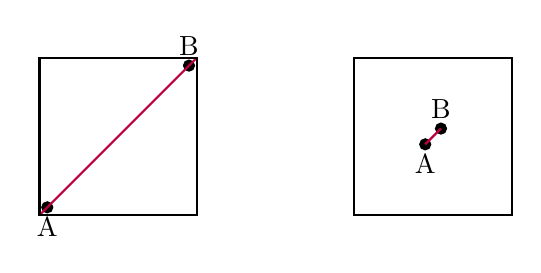
\begin{tikzpicture}

  \filldraw[black] (1.1,1.1) circle (2pt) node[below] {A};
  \filldraw[black] (2.9,2.9) circle (2pt) node[above] {B}; 
  \filldraw[black] (5.9,1.9) circle (2pt) node[below] {A};
  \filldraw[black] (6.1,2.1) circle (2pt) node[above] {B}; 


  % Draw a line between the two dots
  \draw[thick, purple] (1,1) -- (3,3);
  \draw[thick, purple] (5.9,1.9) -- (6.1,2.1);

  % Draw the box
  \draw[thick] (1,1) rectangle (3,3);
  \draw[thick] (5,1) rectangle (7,3);
  
\end{tikzpicture} \\

Question: Cosign distance is not a distance why?
Because it is not nonnegative. 

Question: What's the minimum distance to an edge? \\\\
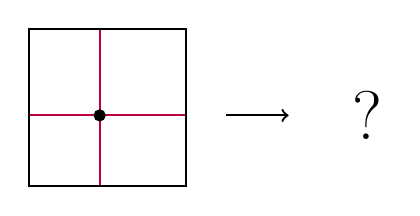
\begin{tikzpicture}


  % Draw a line between the two dots
  \draw[thick, purple] (1.9,3) -- (1.9,1);
  \draw[thick, purple] (3,1.9) -- (1,1.9);

  \filldraw[black] (1.9,1.9) circle (2pt) node[below] {};

  % Draw the box
  \draw[thick] (1,1) rectangle (3,3);

  \draw[->, thick] (3.5, 1.9) -- (4.3, 1.9);
  \node at (5.3, 1.9) {\Huge ?};
  
\end{tikzpicture} \\\\
To find the minimum distance we use norms ($||x||$). There are different types of norms, like:
Euclidean norms\\
Infinity norms\\
$\dots$ \\

\subsection{K-NN}
Meaning: K-NN is K-Nearest Neighbor

How it works: 
\begin{outline}[enumerate]
    \1  Have a data point. 
    \1 Find the distance between the point and all the data points. Euclidean metric is the most common.
    \1 Sort the distances
    \1 Select K Neighbors with the smallest distances from the point.
    \1 Perform the average, or mode.
\end{outline}

Why does it work?

Because not assuming the numbers are uniform will prevent the curse of dimensionality. \\

Class demonstration: Don't follow the pattern\\
\begin{tikzpicture}

  % Draw a graph 
  \draw[thick] (1,5) -- (1,1);
  \draw[thick] (1,1) -- (6,1);

   \filldraw[black] (1.5,2) circle (2pt) node[below] {};
    \filldraw[black] (2,2.5) circle (2pt) node[below] {};
    \filldraw[black] (2.7,2.5) circle (2pt) node[below] {};
    \filldraw[black] (3.2,2) circle (2pt) node[below] {};
    \filldraw[red] (3.8,1.6) circle (2pt) node[below] {};
    \filldraw[black] (4.4,1.8) circle (2pt) node[below] {};
    \filldraw[black] (4.9,2.2) circle (2pt) node[below] {};

    % x1 marker
    \filldraw[purple] (2.4,2) circle (2pt) node[below] {};
    \draw[thick, purple] (2.4,1.2) -- (2.4,1);
    \node[below] at (2.5,1) {\(x_1\)};
    
    % x2 marker
    \node[purple] at (3.3, 3) {\small ?};
    \draw[thick, purple] (3.3,1.2) -- (3.3,1);
    \node[below] at (3.3,1) {\(x_2\)};

    % x3 marker
     \draw[thick, red] (3.8,1.2) -- (3.8,1);
    \node[below] at (3.8,1) {\(x_3\)};

\end{tikzpicture} \\

Limitations: If dimensions increase then it's not Nearest Neighbor. \\

K-NN is used for: 
\begin{itemize}
    \item Binary Classification
    \item Regression
\end{itemize}
Question: What do you do with missing data?

Example:
\[
    \begin{bmatrix}
        1 \\
        ? \\
        3 \\
        4 \\
        7 \\
        ? \\
        5
    \end{bmatrix}
\] 

Methods:
\begin{outline}[enumerate]
    \1 delete it 
    \1 mean or median 
    \1 K-NN (take the nearest neighbors and their average)
\end{outline}

Example: Maine is missing temperature data. Taking the mean won't work since places like Texas and Arizona will effect the results. \\

How to solve this problem? \\
Use K-NN. Do this by taking the temperatures of the closest states and preform the average. 

\textbf{K-NN setup}: 
\[
    \textrm{Data} = D ={(x_i,y_i)}^n \leq \mathbb{R}^px(-1,1)
\]
\[
    x\in \mathbb{R}^p \textrm{ and } y=-1 \textrm{ or } y=1
\]

Rule:
$K$ always needs to be an odd number for classification. This is to prevent a tie from occurring.

Example: Is ? positive or negative? \\
$K = 3$, $p = 2$, $n = 16$

\begin{tikzpicture}

  % Draw a graph 
  \draw[thick] (1,5) -- (1,1);
  \draw[thick] (1,1) -- (6,1);
  
  \node[thick, red] at (3.5, 3) {?};
  \node[black] at (2.1, 2) {-};
  \node[black] at (5, 1.3) {+};
  \node[black] at (1.4, 2.9) {-};
  \node[black] at (5, 4) {-};
  \node[black] at (5, 4) {-};
  \node[black] at (3.5, 4.5) {+};
  \node[black] at (2.3, 2.5) {+};
  \node[black] at (4.5, 2.5) {+};
  \node[black] at (3.3, 1.5) {-};
  \node[circle, draw] at (3.3, 3.5) {-};
  \node[black] at (2.2, 4) {+};
  \node[black] at (2.8, 4.5) {+};
  \node[black] at (1.8, 4.5) {+};
  \node[black] at (1.3, 1.5) {-};
  \node[circle, draw] at (3, 3) {+};
  \node[circle, draw] at (4, 3) {-};
  \node[black] at (3, 2) {-};
   
\end{tikzpicture} 

Answer: The k = 3 closest are a positive negative and negative. Since there are two negatives we assume the ? is negative. \\

Order:
\begin{outline}
    \1 Calculation of distance: $O(np)$
    \1 Sort distances: $O(n log n)$
    \1 Pick k that are the smallest: $O(k)$
\end{outline}

